% !TEX root = thesis_draft.tex

\section{Permutation test analysis}
\label{sec:permutationtest}

\subsection{Introduction}

At this point it is clear how we calculate the raw inter-brain synchrony (IBS)
values, and we have some ideas on how to interprete them. But to
explore how they integrate in a full analysis, we need some task-related
analysis goals to cut our teeth on.

\subsubsection{Task-related research questions}
We decided to determine whether there is an effect of cooperation in
\textcite{newman_effects_2021}'s coordination task on IBS. Assuming there is an
effect, we want to know:

\begin{APAenumerate}
  \item Is the effect of cooperation merely task-dependent (e.g. due to stimuli
  or motor responses), or due to actual interaction within the dyad?
  \item Is there also an effect of the study's manipulation (i.e. varying
  working memory load) on IBS, and how does it develop over time?
  \item Is it possible to predict for new EEG data whether cooperation was
  succesful using just the IBS values?
\end{APAenumerate}

Based on the hyperscanning studies discussed in the introduction, we hypothesize
regarding our task-related research questions that more cooperation will lead to
higher synchrony. We also expect such an effect to not just be caused by the
task but also by the interaction itself. And as a consequence, we expect
prediction of accuracy (i.e. succesful cooperation) on the basis of newly
collected EEG data to also be possible. We expect IBS to vary over time, as at
some point we expect participants to stumble upon a cooperation strategy.
Finally, we hypothesize high working memory load to be detrimental to IBS
because of \textcite{maehara_i_2011,newman_effects_2021}'s behavioural results.

While most of the task-related questions we plan to answer have an exploratory
nature, we also have one directly testable hypothesis: we expect IBS in frontal
and temperoparietal areas in the alpha band \parencite{newman_effects_2021}.
This hypothesis is based on the findings of
\textcite{van_vugt_inter-brain_2020}. They found ``frontal alpha oscillations''
during ``moments of agreement'' in monastic debate. And also on the findings of
\textcite{hu_inter-brain_2018}, who found higher (phase locking value) synchrony
in the alpha band in centro-parietal regions during high cooperation than low
cooperation.

\subsection{Methods}

The task-dependent and dyad-dependent effects on IBS are tested separately,
the former by running a permutation test against shuffled samples and the latter
by running a permutation test against virtual dyads assembled from random
participants that never performed the task together.

% NOTE: these are included early because a lot of figures follow in a small
% amount of text
\begin{figure}[!htpb]
  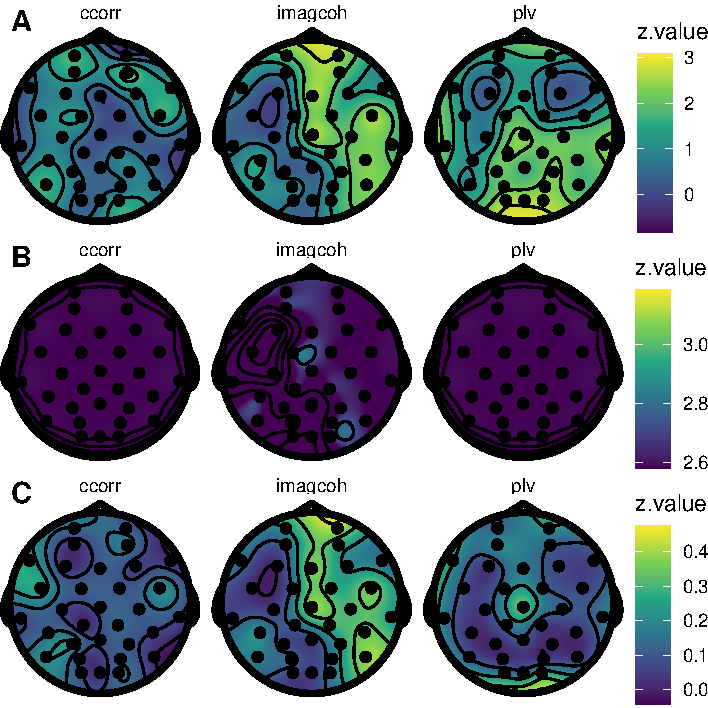
\includegraphics[width=\linewidth]{../stats/results/permutation_alpha.pdf}
  \caption{Is there an effect of the task (A, B) or the within-dyad interaction (C) on IBS in the alpha (9--14 Hz) band? After FDR correction, most values in (B) meet the significance threshold, which in that case lies at 2.58. But (B), which shuffles the spectrum instead of the original data (A), does not visualize a valid permutation test (see text). Other tests do not meet the significance threshold.}
  \label{fig:permutation_alpha}
\end{figure}

\begin{figure}[!htpb]
  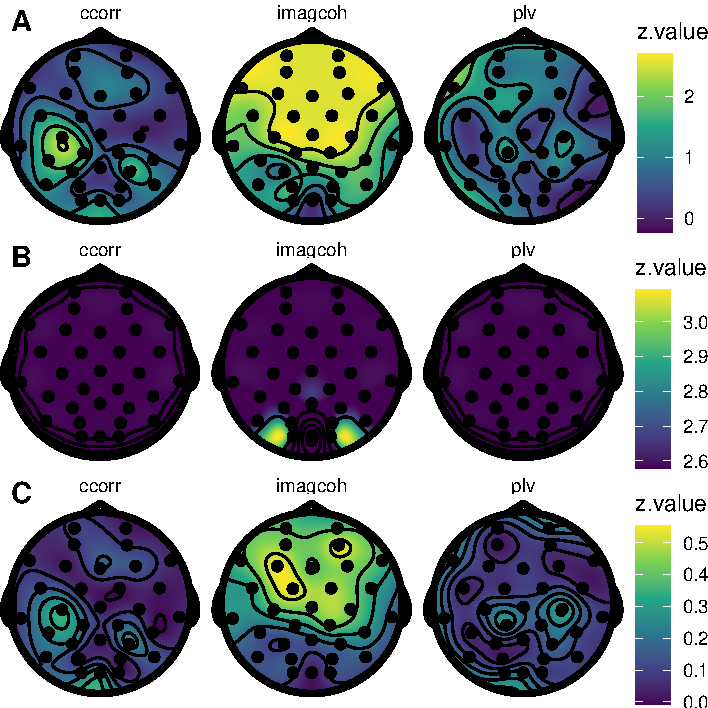
\includegraphics[width=\linewidth]{../stats/results/permutation_theta.pdf}
  \caption{Is there an effect of the task (A, B) or the within-dyad interaction (C) on IBS in the theta (4--7 Hz) band? After FDR correction, most values in (B) meet the significance threshold, which in that case lies at 2.58. But (B), which shuffles the spectrum instead of the original data (A), does not visualize a valid permutation test (see text). Other tests do not meet the significance threshold.}
  \label{fig:permutation_theta}
\end{figure}

By shuffling samples, we force the recording of one participant to be
independent from the recording of the other participant as they no longer match
up in time \parencite{lachaux_measuring_1999}. This also destroys any effects of
(temporal) task structure. There is a problem though: there are multiple ways to
shuffle samples. We can shuffle the original signal or the frequency spectrum.
If we could convert between the time and frequency domain at any resolution,
both approaches would be equivalent. But as we have previously seen in this
study, phase and amplitude information is in practice estimated over time
windows of up to a second. We run both tests to determine the differences in
practise. The permutation tests use 200 repetitions.

By shuffling dyads, we can determine whether there is something that makes the
IBS values of actual dyads different compared to randomly assembled dyads that
were never actually cooperating. As each participant saw the same stimuli in
\textcite{newman_effects_2021}'s experiment (albeit in a different order), it is
possible to construct virtual dyads such that they still saw the same stimuli.
This prevents the permutation test from detecting effects that are actually due
to the stimuli instead of the participants themselves. For this permutation
test, all possible combinations of virtual dyads are generated. As the amount of
participants is limited, this is computationally feasible.

The result of a permutation test is a large data set that has an IBS value for
each IBS measure, session, electrode, trial and permutation test repetition. We
first average out trial, then session resulting in a distribution for each
measure and electrode. Using the same averaging on the actually observed data,
we get a single value to compare each distribution against. We calculate a
p-value from this by looking how extreme this value is compared to the
distribution \parencite[see][for a robust method]{phipson_permutation_2010}.
We convert these p-values to z-scores when visualizing the results, to make any
colour transitions more gradual.

Because we perform comparisons for each measure and electrode, we control the
false discovery rate (FDR) using a \textcite{benjamini_controlling_1995}
procedure and report the resulting threshold.

\subsection{Results}

To assess whether there is an effect of the task, we perform a permutation test
where we shuffle the EEG timeseries data within trials before calculating IBS.
When we shuffle in the time domain (panel (A) in
Figures~\ref{fig:permutation_alpha}~\&~\ref{fig:permutation_theta}), we find no
significant effect. When we instead shuffle in the frequency domain, we appear
to find a significant effect almost everywhere on the scalp for all the measures
(panel (B) in Figures~\ref{fig:permutation_alpha}~\&~\ref{fig:permutation_theta}).
The only exceptions are for the imaginary part of coherency measure, which is
not significant after FDR correction for the Oz electrode in the theta band and
the F3, FC5, T7, C3, P3, Pz, O1 and Oz electrodes in the alpha band.

\begin{figure}[!htpb]
  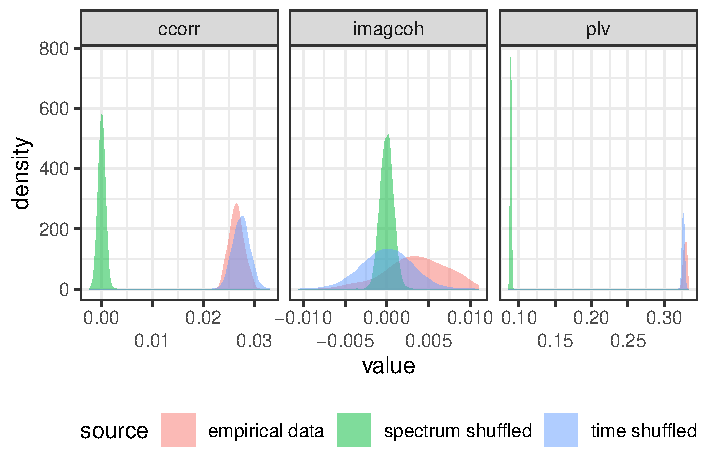
\includegraphics[width=\linewidth]{../stats/results/shuffledistributions.pdf}
  \caption{Shuffling the frequency spectrum is not equivalent to shuffling the underlying time series and then estimating the spectrum. Clearly, the shortcut of shuffling the spectrum results in a less conservative test.}
  \label{fig:shuffledistributions}
\end{figure}

\begin{figure}[!htpb]
  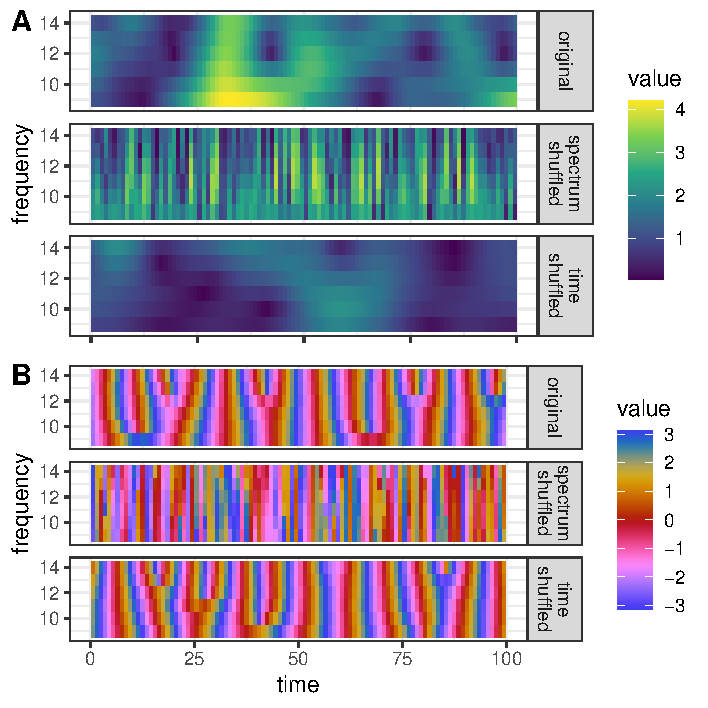
\includegraphics[width=\linewidth]{../stats/results/shufflecompare.pdf}
  \caption{An example of an original spectrum (identical to Figure~\ref{fig:freqanalysis}B \& C), the same spectrum but shuffled, and a spectrum generated from the same data but shuffled before frequency analysis. Spectrum amplitudes (A) and phases (B) are shown.}
  \label{fig:shufflecompare}
\end{figure}

Considering we could not find a task-related effect on IBS when shuffling the
time series data, it is not surprising that the tests for a within-dyad
interaction effect are also insignificant for all electrodes and measures
(panel~(C) in
Figures~\ref{fig:permutation_alpha}~\&~\ref{fig:permutation_theta}). After all,
it tests a more specific claim: whether there is an effect of working together.

\subsection{Discussion}

The difference in significance in panels (A) and (B) of
Figures~\ref{fig:permutation_alpha}~\&~\ref{fig:permutation_theta}) is because
the permutation test null distributions differ depending on the shuffling method
(see Figure~\ref{fig:shuffledistributions}). Shuffling the spectrum results in a
less conservative test. When we look at the difference between the spectra
(Figure~\ref{fig:shufflecompare}), it becomes clear that the frequency analysis
process normally results in a smoothed spectrum. But also, that this is not the
case when the spectrum is shuffled. As a result, this method of generating a
permutation test null distribution should not be used. It results in an invalid
test.

Contrary to our expectations, we found neither a task-dependent nor a
dyad-dependent effect of on IBS. As a result, testing whether this effect varies
by level of cooperation (i.e. presumably accuracy), working memory load or over
time does not make much sense. For the purpose of exploring the full IBS
pipeline, the next two sections will make an attempt regardless by analysing the
time course and trying to predict accuracy from the IBS values.

We also expected IBS in frontal and temperoparietal areas for the alpha band. No
such effect was found.
